\section{Container}

\subsection{Docker}

Docker is a software platform that enables applications and their dependencies to be packaged into  environments called containers.

\begin{figure}[htb]
  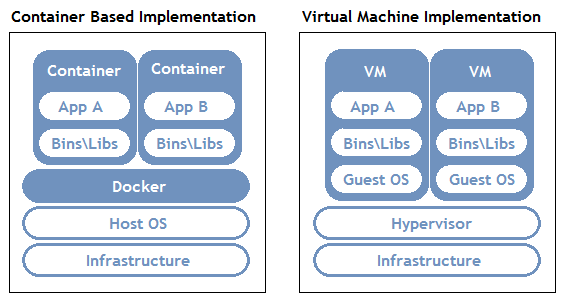
\includegraphics[width=\linewidth]{images/docker.png}
  \caption{Architecture of Docker vs. a standard VM}
\end{figure}

In order to facilitate Docker-related tasks on multiple machines, we developed a command line tool that:

\begin{enumerate}
    \item Installs Docker on one or more Linux hosts in parallel.
    \item Acts as an orchestration layer for the Docker-equipped hosts by exposing a single API to run Docker commands on more than one host simultaneously.
\end{enumerate}

Since Docker containers include a stripped-down version of a Linux distribution, they have everything they need to run on any machine that supports Docker, regardless of the Host OS. This makes Docker an ideal tool for benchmarking multi-cloud services. If the benchmarking script runs on one cloud, whether that's AWS, GCP, or a private cloud running on a cluster of Raspberry Pi devices, it runs on them all.

\subsection{Kubernetes}

Kubernetes \cite{www-kubernetes} is a powerful, open source container orchestration system. We have set up a singular master node, and five worker nodes that each can host a container image. Each worker will be able to handle a number of pods (or components) that will be distributed by the master.

\begin{figure}[htb]
  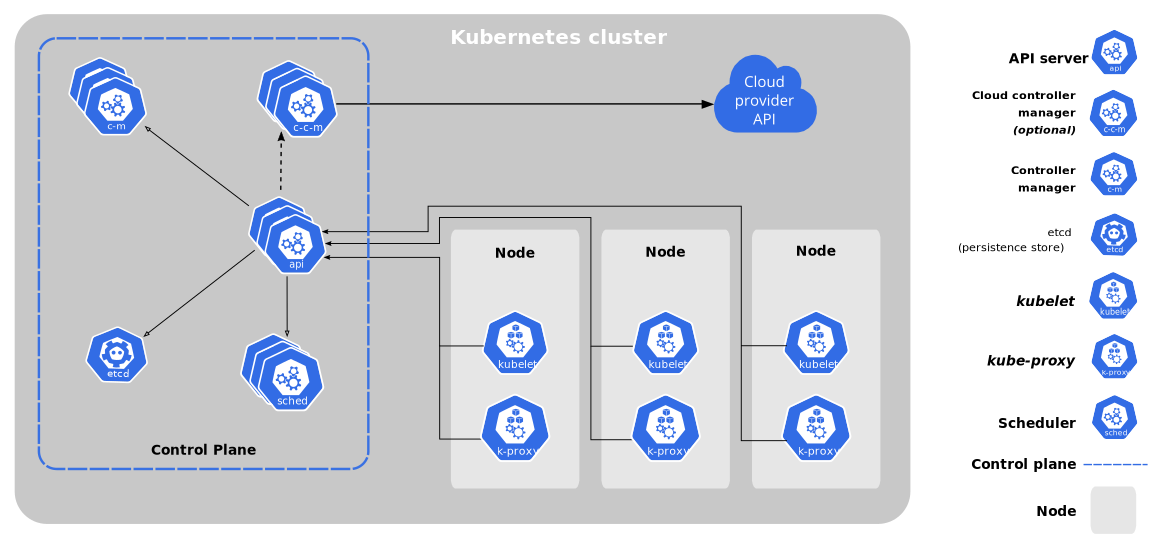
\includegraphics[width=\linewidth]{images/cluster_image.png}
  \caption{Example Cluster Setup \cite{kubernetes-image}}
\end{figure}

\subsubsection{Kubernetes Flavors}
There are multiple Kubernetes flavors that have been developed that have differnet utilities based on the specific application. For example, Minikube is a powerful Kubernetes flavor that is useful to deploy locally, but serves no purpose with a cluster setup (like the one we created). Some other popular alternatives include Ubuntu, K8s, MicroK8s, and K3S. 

We settled on implementing K3s for a few reasons:

\begin{enumerate}
    \item Self-branded as a "lightweight Kubernetes," it was much more feasible to run on our small memory RPi's (ie. RPi 3B+ had 1 GB of RAM)
    \item Small sized package (<40 MB binary file)
    \item Optimized for ARM-based devices (which the RPi's are)
\end{enumerate}

\subsubsection{Design}
We created three different clusters that consisted of one Raspberry Pi 4 master node and five Raspberry Pi 3B+ worker nodes. By enabling these clusters, we gave ourselves the ability to easily scale containerization and use this to run across the cluster at any specified amount of iterations. Since Kubernetes automates away many of the manual (and labour intensive) tasks involved with scaling up/down containers —  in our case, the ones we developed in Docker — we allowed ourselves to devote more time and resources towards designing and implementing the actual Python programs.




\subsection{Containers and Microservices}
\label{containers-and-microservices}

Cloudmesh uses the internet architectures of microservices and
containers to organize its functions and code. Microservice architecture
is a variant of service oriented architecture. Cloudmesh uses
microservices to arrange its app in loosely coupled services. These
services are fine grained and protocals are lightweight. Containers are
data structures whose instances are collections of other objects.
Cloudmesh uses containers to store objects in an organized way that
follows specific access rules. Containers are characterized by three
properties: accessing objects in the container, storage of the objects,
and traversal of the objects. Cloudmesh is designed to work on
containers in docker, and kubernetes.

\TODO{THIS SHOULD BE CITATION}

 \url{https://opensource.com/article/20/3/kubernetes-raspberry-pi-k3s}
